\subsection{Kamera}
Als weiteren Baustein der Android-App wird eine Kamera benötigt. Es stehen zurzeit 
zwei Kamera Frameworks von Android zur Verfügung. Das eine Framework ist die (deprecated)‚ 
\enquote{Camera}, die seit dem Android API-Level\footnote{Application Programming Interface} 1 Teil des 
Android Development Kits (ADK) ist.
%
\begin{figure}[h!]
	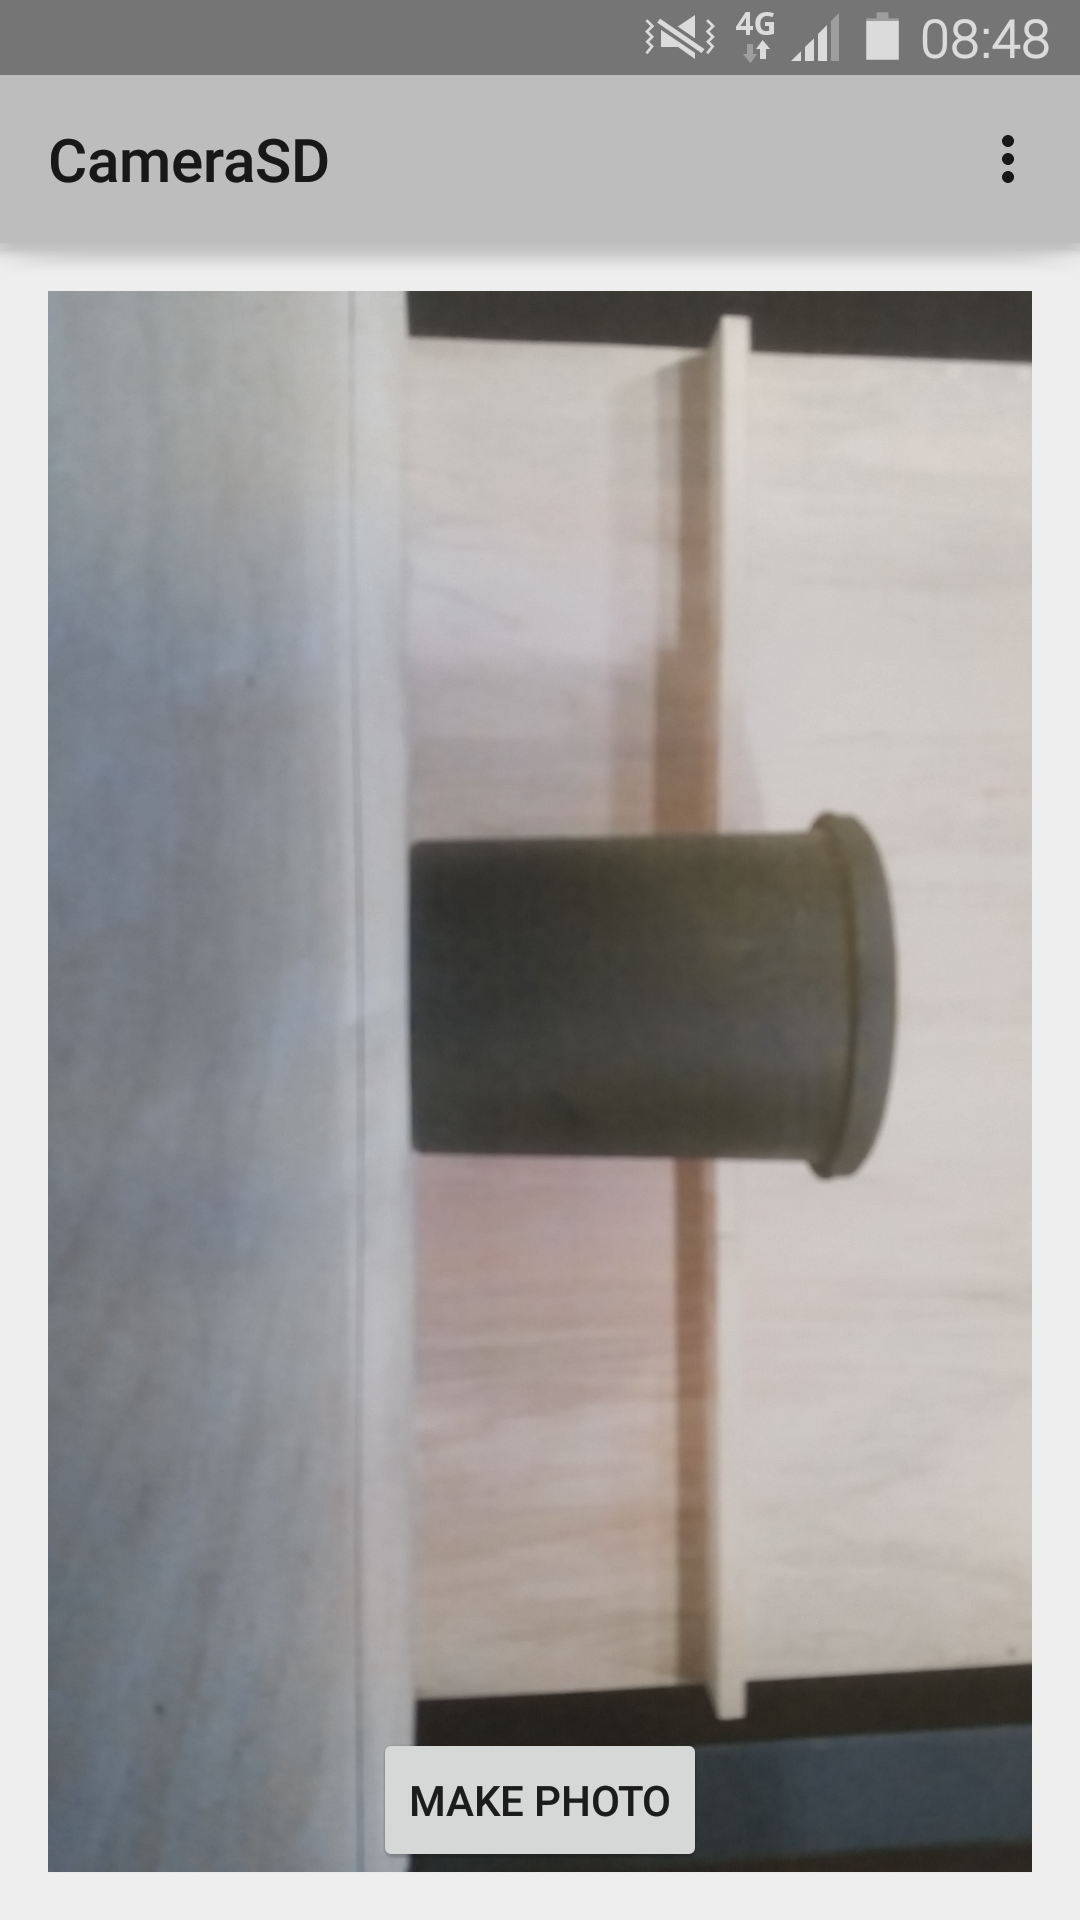
\includegraphics[width=0.3\textwidth,clip,trim=0mm 0mm 0mm 0mm]
	{Enddokumentation/Bilder/Screenshot_CameraSD.png}
	\centering
	\caption{Screenshot Camera Prototypen-App}
	\label{abb:ScreenshotCameraSD}
\end{figure}
%
Das andere Framework ist die Neue, ab API Level 21 verfügbare‚ 
\enquote{Camera2}. Um die beiden Camera-Typen zu untersuchen, testen und vergleichen, wurden je eine Test-App programmiert.
Im Vergleich der beiden Frameworks zeigte sich, dass die Entwicklung einer App mit dem alten Camera-Typ 
einiges speditiver von statten geht und der Code viel verständlicher ist. Die Entscheidung fiel deshalb 
auf das zwar veraltete aber erprobte  \enquote{Camera}-Framework.
\newline
\newline
Erst nach dem Test der beiden Applikationen konnte das Informatik-Team das Gerät für den PREN-Wettkampf festlegen. 
Da dieses Gerät auf Android Jelly Bean (API Level 17) basiert, schliesst dies die Verwendung 
der  \enquote{Camera2} (ab API Level 21) aus.
